\chapter{Prawdopodobieństwo i funkcje straty}\label{rozdz:strata}

\section{Jak powiedzieć modelowi, że się myli?}

Wyjściem sieci jest, dla każdej klatki i półtonu, liczba z przedziału $(0,1)$: „z jakim prawdopodobieństwem w tej klatce gra ta nuta?”.
Żeby uczyć sieć gradientem (rozdział~\ref{rozdz:pochodne}), potrzebujemy funkcji straty: jednej liczby, która jest mała, gdy odpowiedzi
są dobre, i duża, gdy złe. Tu wyprowadzimy dwie funkcje używane w Gen~6 (sigmoidę z entropią krzyżową dla początków, ramek i końców; softmax dla tabulatury)
i pokażemy, \emph{dlaczego} akurat takie.

Po tym rozdziale umiesz: (i)~zamienić liczbę rzeczywistą na prawdopodobieństwo sigmoidą i softmaksem, (ii)~policzyć stratę BCE i jej gradient,
(iii)~uzasadnić, że BCE jest najmniejsza dla prawdziwego prawdopodobieństwa, (iv)~powiedzieć, co robi waga klasy dodatniej.

\section{Sigmoida i softmax}

\haslo{sigmoida}
\begin{definicja}[Sigmoida]\label{def:sigmoida}
Funkcja $\sigma(z)=\dfrac1{1+e^{-z}}$ przekształca dowolną liczbę $z\in\R$ (zwaną \emph{logitem}) w liczbę z przedziału $(0,1)$.
Zachodzi $\sigma(-z)=1-\sigma(z)$ i $\sigma(0)=\tfrac12$.
\end{definicja}

\begin{przyklad}\label{prz:sigmoida}
$\sigma(0)=0{,}5$; $\sigma(2)=0{,}881$; $\sigma(-2)=0{,}119$; $\sigma(-3)=0{,}0474$. Duży dodatni logit oznacza „prawie na pewno tak”, duży ujemny
„prawie na pewno nie”. Odwrotność: $z=\ln\frac{p}{1-p}$ (logarytm szans).
\end{przyklad}

\haslo{softmax}
\begin{definicja}[Softmax]\label{def:softmax}
Dla wektora logitów $\vect z\in\R^K$ (K klas) \emph{softmaksem} nazywamy wektor o współrzędnych
$\softmax(\vect z)_i=\dfrac{e^{z_i}}{\sum_{j=1}^{K}e^{z_j}}$.
\end{definicja}

\begin{przyklad}\label{prz:softmax}
Dla $\vect z=(2;1;0{,}1)$ mamy $e^{z}=(7{,}389;\,2{,}718;\,1{,}105)$, suma $11{,}212$, więc softmax to $(0{,}659;\,0{,}242;\,0{,}099)$.
Największy logit dostaje największe prawdopodobieństwo, ale mniejsze też nie giną.
\end{przyklad}

\begin{twierdzenie}[Własności softmaksa]\label{tw:softmax}
Dla każdego $\vect z$: (a) $\softmax(\vect z)_i>0$ i $\sum_i\softmax(\vect z)_i=1$; (b) $\softmax(\vect z+c\vect 1)=\softmax(\vect z)$ dla dowolnej stałej $c$.
\end{twierdzenie}
\begin{pomyslDowodu}
(a) wynika z dodatniości wykładnika i z tego, że dzielimy przez sumę; (b): czynnik $e^c$ skraca się w liczniku i mianowniku.
\end{pomyslDowodu}
\begin{proof}
(a) $e^{z_i}>0$ dla każdego $z_i$, a mianownik jest sumą takich liczb, więc wynik jest dodatni; suma ułamków o wspólnym mianowniku $\sum_j e^{z_j}$ daje $1$.
(b)
\begin{align*}
\frac{e^{z_i+c}}{\sum_j e^{z_j+c}} &= \frac{e^{c}e^{z_i}}{e^{c}\sum_j e^{z_j}} && \pow{($e^{a+b}=e^ae^b$)}\\
 &= \frac{e^{z_i}}{\sum_j e^{z_j}}. && \pow{(skrócenie $e^c$)}
\end{align*}
W praktyce odejmujemy od logitów ich maksimum ($c=-\max z$), żeby uniknąć przepełnienia $e^{z}$ dla dużych $z$ --- wynik się nie zmienia. To kończy dowód.
\end{proof}

Sigmoida to softmax dwóch klas $(z,0)$: $\softmax(z,0)_1=e^z/(e^z+1)=\sigma(z)$. Używamy sigmoidy, gdy klasy nie wykluczają się (w jednej klatce może grać wiele półtonów naraz), a softmaksu, gdy
dokładnie jedna odpowiedź jest prawdziwa (na strunie dokładnie jedna z $21$ klas: milczy albo któryś próg).

\section{Entropia krzyżowa}

\haslo{entropia krzyżowa}
\begin{definicja}[Strata BCE]\label{def:bce}
Dla prawdopodobieństwa $p\in(0,1)$ i etykiety $y\in[0,1]$ (zwykle $0$ lub $1$) \emph{binarna entropia krzyżowa} wynosi
\begin{equation}
  \ell(p,y)=-\big[\,y\ln p+(1-y)\ln(1-p)\,\big].
\end{equation}
Z \emph{wagą klasy dodatniej} $\alpha>0$: $\ell_\alpha(p,y)=-\big[\alpha\,y\ln p+(1-y)\ln(1-p)\big]$.
\end{definicja}

\begin{przyklad}\label{prz:bce}
Dla $y=1$ i $p=0{,}9$: $\ell=-\ln0{,}9=0{,}105$. Dla $p=0{,}2$: $\ell=-\ln0{,}2=1{,}609$; z wagą $\alpha=4$ strata wynosi $6{,}44$. Dla $y=0$ i $p=0{,}2$: $\ell=-\ln0{,}8=0{,}223$.
Pewność w złą stronę ($p\to0$ przy $y=1$) jest karana nieograniczenie: $-\ln p\to\infty$ (rys.~\ref{rys:bce}a).
\end{przyklad}

\begin{intuicja}
Strata BCE to „zaskoczenie” modelu: $-\ln p$ to ile bitów (nat) informacji niesie zdarzenie, któremu przypisaliśmy $p$. Model, który
był pewien złej odpowiedzi, jest bardzo zaskoczony, więc ponosi dużą karę.
\end{intuicja}

\begin{twierdzenie}[Gradient BCE po logicie]\label{tw:grad-bce}
Dla $p=\sigma(z)$: $\dfrac{\partial\ell}{\partial z}=\sigma(z)-y$. Z wagą $\alpha$: $\dfrac{\partial\ell_\alpha}{\partial z}=(\alpha y+1-y)\,\sigma(z)-\alpha y$.
\end{twierdzenie}
\begin{pomyslDowodu}
Regułą łańcuchową przez $p=\sigma(z)$ i pochodną sigmoidy $\sigma'=\sigma(1-\sigma)$ (tw.~\ref{tw:pochodna-sigmoidy}); czynniki $p(1-p)$ się skracają.
\end{pomyslDowodu}
\begin{proof}
Niech $p=\sigma(z)$, więc $\partial p/\partial z=p(1-p)$. Dla $\ell_\alpha$:
\begin{align*}
\frac{\partial\ell_\alpha}{\partial p} &= -\frac{\alpha y}{p}+\frac{1-y}{1-p} && \pow{(pochodna $\ln$)}\\
\frac{\partial\ell_\alpha}{\partial z} &= \Big(-\frac{\alpha y}{p}+\frac{1-y}{1-p}\Big)p(1-p) && \pow{(reguła łańcuchowa)}\\
 &= -\alpha y(1-p)+(1-y)p && \pow{(skrócenie)}\\
 &= (\alpha y+1-y)\,p-\alpha y. && \pow{(wyłączenie $p$)}
\end{align*}
Dla $\alpha=1$ to $p-y$. Dla $y=1$ gradient to $-\alpha(1-p)$, dla $y=0$ to $p$. To kończy dowód.
\end{proof}

W zwykłym języku: gradient po logicie to po prostu „odpowiedź modelu minus prawda”. Gdy $y=1$ i model mówi $p\approx0$ (bardzo się myli), gradient jest bliski $-1$ --- silny sygnał do poprawy.
Dla błędu kwadratowego $(p-y)^2$ ten sam gradient to $2(p-y)p(1-p)$, który \emph{znika}, gdy sigmoida jest nasycona
(rys.~\ref{rys:bce}b): np.\ dla $z=-5$ i $y=1$ gradient BCE wynosi $-0{,}993$, a błędu kwadratowego tylko $-0{,}013$. Dlatego do klasyfikacji używamy BCE.

\begin{figure*}[ht]
\centering
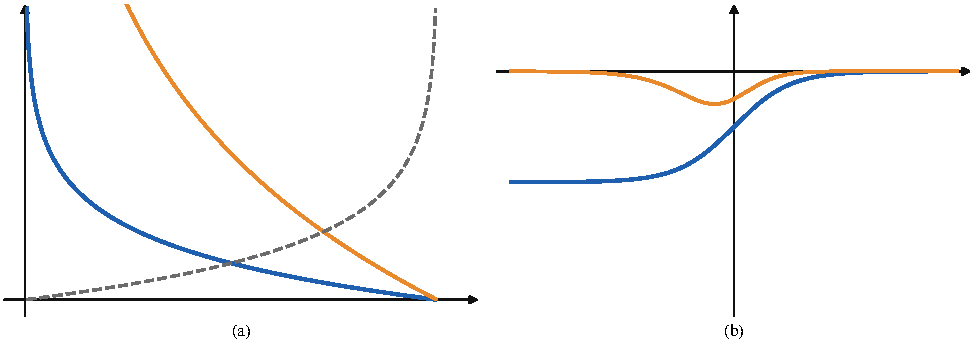
\includegraphics[width=\linewidth]{figures/bce.pdf}
\caption{(a) Strata BCE w funkcji $p$: dla $y=1$ ($-\ln p$, niebieska) i z wagą $\alpha=4$ (pomarańczowa) rośnie do nieskończoności, gdy $p\to0$; dla $y=0$ ($-\ln(1-p)$, szara przerywana)
rośnie, gdy $p\to1$. (b) Gradient po logicie dla $y=1$: BCE (niebieska, $\sigma-1$) pozostaje blisko $-1$ przy dużym błędzie; gradient błędu kwadratowego (pomarańczowa) zanika w nasyceniu.}
\label{rys:bce}
\end{figure*}

\begin{twierdzenie}[BCE uczy prawdziwego prawdopodobieństwa]\label{tw:kalibracja}
Niech etykieta $y\in\{0,1\}$ wypada $1$ z prawdopodobieństwem $q\in(0,1)$. Średnia strata $\Exp[\ell_\alpha(p,y)]=-\alpha q\ln p-(1-q)\ln(1-p)$ jest najmniejsza dla
\begin{equation}
  p^\ast=\frac{\alpha q}{\alpha q+1-q}.
\end{equation}
W szczególności dla $\alpha=1$ jest to $p^\ast=q$.
\end{twierdzenie}
\begin{pomyslDowodu}
Różniczkujemy średnią stratę po $p$, przyrównujemy do zera i sprawdzamy, że to minimum.
\end{pomyslDowodu}
\begin{proof}
Niech $J(p)=-\alpha q\ln p-(1-q)\ln(1-p)$ dla $p\in(0,1)$.
\begin{align*}
J'(p) &= -\frac{\alpha q}{p}+\frac{1-q}{1-p}=0 && \pow{(warunek konieczny)}\\
\Rightarrow\;\alpha q(1-p) &= (1-q)p \;\Rightarrow\; p^\ast=\frac{\alpha q}{\alpha q+1-q}. && \pow{(rozwiązanie względem $p$)}
\end{align*}
Druga pochodna $J''(p)=\alpha q/p^2+(1-q)/(1-p)^2>0$, więc to jedyne minimum. To kończy dowód.
\end{proof}

\begin{naliczbach}
Jeśli w danym półtonie początek nuty występuje w $q=10\%$ przypadków, a waga to $\alpha=4$, model uczony BCE nauczy się mówić $p^\ast=0{,}4/(0{,}4+0{,}9)=0{,}308$, a nie $0{,}1$. Waga zawyża więc prawdopodobieństwa
(rys.~\ref{rys:kalibracja}). Podobnie miękka etykieta $y=0{,}4$ (sąsiednie klatki wokół początku w Gen~6) przy $\alpha=1$ i $q$ interpretowanym jako średnia etykieta daje $p^\ast=0{,}4$: model nie jest karany
za niepewność o jedną klatkę.
\end{naliczbach}

\begin{figure}[ht]
\centering
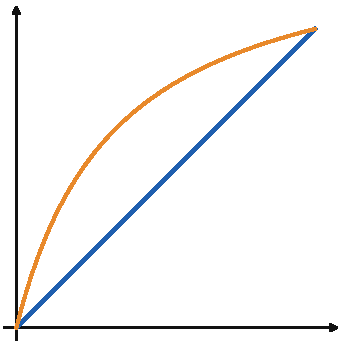
\includegraphics[width=\linewidth]{figures/kalibracja.pdf}
\sidecaption{Optymalne prawdopodobieństwo $p^\ast$ (pion) w zależności od prawdziwej częstości $q$ (poziom) dla wagi $\alpha=1$ (niebieska, leży na przekątnej) i $\alpha=4$ (pomarańczowa, nad przekątną). Waga klasy dodatniej
przesuwa wyjścia sieci w górę; dekoder (rozdział~\ref{rozdz:dekoder}) musi to uwzględnić przez progi dobrane na walidacji. \label{rys:kalibracja}}
\end{figure}

\begin{pulapka}
Wyjścia sieci uczonej z wagą $\alpha>1$ \emph{nie są} prawdziwymi prawdopodobieństwami. Próg $0{,}5$ w dekoderze nie ma wtedy żadnego szczególnego znaczenia; dlatego progi dekodera Gen~6 stroimy osobno (rozdział~\ref{rozdz:dekoder}).
\end{pulapka}

\section{Dlaczego rzadkie etykiety są trudne}

Weźmy prawdziwy przykład: nagranie z rozdziału~\ref{rozdz:hcqt} ($T=243$ klatek, $53$ półtony, $12\,879$ komórek) ma $15$ nut. Mapa początków ma więc tylko $15$ komórek równych $1$ (i $30$ równych $0{,}4$): to $0{,}12\%$ wszystkich.
Sieć, która zawsze odpowiada „zero”, ma niemal idealną dokładność, a zupełnie nie nadaje się do niczego. Dwa środki zaradcze używane w Gen~6: waga $\alpha=4$ dla początków ($\alpha=2$ dla końców) oraz
\emph{inicjalizacja obciążenia} ostatniej warstwy na $-3$ dla początków (i $-2$ dla ramek). Na starcie $\sigma(-3)=0{,}047$, więc strata na komórkę to $-\big[0{,}0012\ln0{,}047+0{,}9988\ln0{,}953\big]=0{,}052$,
a przy $\sigma(0)=0{,}5$ byłoby $0{,}693$: sieć nie musi tracić pierwszych kroków na samo „nauczenie się, że nut jest mało”.

\section{Softmax i tabulatura}

Dla jednej struny w jednej klatce sieć zwraca $21$ logitów (klasa $0$: struna milczy, klasy $1+f$ dla progów $f=0,\dots,19$). Strata to ujemny logarytm prawdopodobieństwa klasy prawdziwej:
$\ell=-\ln\softmax(\vect z)_c=-z_c+\ln\sum_je^{z_j}$. Jej gradient po logitach to $\softmax(\vect z)-\vect e_c$ (analogicznie do tw.~\ref{tw:grad-bce}).

\begin{naliczbach}
Dla trzech klas $\vect z=(2;1;0{,}1)$ i prawdziwej klasy $c=1$ (pierwszej): $\softmax=(0{,}659;\,0{,}242;\,0{,}099)$, strata $-\ln0{,}659=0{,}417$, gradient po logitach $(0{,}659-1;\ 0{,}242;\ 0{,}099)=(-0{,}341;\ 0{,}242;\ 0{,}099)$.
Zwróćmy uwagę: suma gradientu to zero, bo suma softmaksu to $1$ --- podnoszenie jednego logitu odbywa się kosztem pozostałych.
\end{naliczbach}

\section*{Podsumowanie}
\begin{itemize}
\item $\sigma$ zamienia logit na prawdopodobieństwo; softmax robi to dla wielu wykluczających się klas i jest niezmienniczy względem dodania stałej.
\item BCE $=-[y\ln p+(1-y)\ln(1-p)]$; jej gradient po logicie to $\sigma(z)-y$ (tw.~\ref{tw:grad-bce}).
\item BCE jest najmniejsza dla prawdziwej częstości; waga $\alpha$ zawyża wyjścia do $\frac{\alpha q}{\alpha q+1-q}$ (tw.~\ref{tw:kalibracja}).
\item Etykiety początków są rzadkie ($0{,}12\%$ komórek), więc używamy wagi i obciążenia początkowego $-3$.
\item Tabulatura: softmax po $21$ klasach na strunę i strata $-\ln p_{\mathrm{klasa}}$.
\end{itemize}

\begin{sprawdz}
\begin{enumerate}
\item Policz $\sigma(1)$, $\sigma(-1)$ i sprawdź, że sumują się do $1$.
\item Dla $y=1$ policz stratę BCE z $\alpha=1$ oraz $\alpha=2$ przy $p=0{,}3$, a także gradient po logicie w obu przypadkach.
\item Pokaż, że $\softmax(z,0)_1=\sigma(z)$.
\item Przy $q=0{,}05$ i $\alpha=2$ ile wynosi $p^\ast$? Jaką wagę $\alpha$ trzeba wziąć, by $p^\ast=0{,}5$ przy $q=0{,}05$?
\end{enumerate}
\end{sprawdz}

\subsection*{Rozwiązania}
\begin{enumerate}
\item $\sigma(1)=0{,}7311$, $\sigma(-1)=0{,}2689$, suma $1{,}0000$.
\item $\alpha=1$: $-\ln0{,}3=1{,}204$, gradient $0{,}3-1=-0{,}7$. $\alpha=2$: strata $2{,}408$, gradient $-2(1-0{,}3)=-1{,}4$.
\item $\softmax(z,0)_1=e^{z}/(e^{z}+e^{0})=e^{z}/(e^{z}+1)=1/(1+e^{-z})=\sigma(z)$ (dzielimy licznik i mianownik przez $e^{z}$).
\item $p^\ast=2\cdot0{,}05/(0{,}1+0{,}95)=0{,}095$. Z równania $\alpha q=1-q$: $\alpha=(1-q)/q=19$ daje $p^\ast=0{,}5$.
\end{enumerate}
